\chapter{Handleiding voor ontwikkelaars}
\label{appendix-e}

Deze handleiding is bedoeld voor ontwikkelaars en bestaat uit twee delen. Het eerste deel is bedoeld voor mensen die de synchronisatiebibliotheek willen gebruiken in eigen projecten zonder de broncode te wijzigen. Het tweede deel legt uit hoe de bibliotheek aangepast kan worden.

Het volledige project is openbaar beschikbaar op \url{https://github.com/wardva/SignalSync}. Het Java-project bevindt zich in de map \textbf{SignalSync}.

\section{Gebruiken van de broncode}

\subsection*{De softwarebibliotheek importeren in Eclipse}

Vooraleer er van start kan worden gegaan moeten de bestanden \texttt{config.properties}, \texttt{signalsync.jar}\footnote{Het JAR bestand bevat ook alle afhankelijkheden: Panako\cite{six2014panako}, TarsosDSP\cite{six2014tarsosdsp} en TeensyDAQ.} en de jSSC JAR bestanden gedownload worden van het volgende (publieke) GitHub repository: \url{https://github.com/wardva/SignalSync/tree/master/Dist}. Deze bestanden bevinden zich ook in een Zip bestand dat rechtstreeks gedownload kan worden van volgende URL: \url{https://github.com/wardva/SignalSync/raw/master/Dist/SignalSync.zip}

Maak vervolgens het Java-project aan in Eclipse dat gebruik zal maken van de softwarebibliotheek. Ga hierna naar de properties van het project, selecteer links \textbf{Java Build Path} en klik op de tab \textbf{Libraries}. Klik vervolgens op de knop \textbf{Add External JARs}. Ga nu op zoek naar \texttt{signalsync.jar}, \texttt{jssc.jar} en \texttt{jssc-2.7.0-src.jar} en voeg ze toe aan het project. Let erop dat het configuratiebestand zich steeds in dezelfde map bevindt als de JAR bestanden.

\subsection*{Broncode en documentatie koppelen aan project}

\texttt{signalsync.jar} bevat de broncode en Javadoc van de softwarebibliotheek. Deze bestanden kunnen aan een bestaand Eclipse project gekoppeld worden waardoor het mogelijk wordt om tijdens het ontwikkelen gebruik te maken van deze informatie. Dit kan worden verwezenlijkt door in de eerder besproken \textbf{Libraries} tab op zoek te gaan naar \texttt{signalsync.jar} en dit item uit te klappen. 

\subsubsection{Koppelen van de broncode}

Selecteer \textbf{Source attachment} en klik op \textbf{edit}. Selecteer \textbf{External location} en ga vervolgens op zoek naar \texttt{signalsync.jar}.

\subsubsection{Koppelen van de Javadoc}

Selecteer \textbf{Javadoc location} en klik op \textbf{edit}. Selecteer \textbf{Javadoc in archive}. Blader vervolgens bij \textbf{Archive path} naar de locatie van \texttt{signalsync.jar}. Blader en selecteer bij \textbf{Path within archive} het mapje \textbf{doc} in het JAR bestand.

\section*{Aanmaken en synchroniseren van streams}

Hoe de streams aangemaakt en gesynchroniseerd kunnen worden is het gemakkelijkst uit te leggen aan de hand van een voorbeeld. In het voorbeeld worden enkele streams aangemaakt en wordt de latency ertussen bepaald. Meer informatie over de TarsosDSP \texttt{AudioDispatchers} is te vinden in artikel \cite{six2014tarsosdsp}.

Om te beginnen moeten er enkele streams worden aangemaakt. In dit voorbeeld zal gebruik gemaakt worden van \texttt{AudioDispatcherStreams}. \\

\lstset{basicstyle=\footnotesize,style=javaStyle}

\begin{lstlisting}
//Een AudioDispatcher aanmaken van een microfoon
AudioDispatcher micDispatcher =
	AudioDispatcherFactory.fromDefaultMicrophone(512, 0);

//AudioDispatcher wrappen in een Stream
Stream micStream = 
	new AudioDispatcherStream(micDispatcher);

//Datastream koppelen aan microfoon
Stream dataStreamAttachedToMicrophone = ...

//Een AudioDispatcher aanmaken van een bestand
File file = new File("recorded.wav");
AudioDispatcher fileDispatcher = 
	AudioDispatcherFactory.fromFile(file, 512, 0);

//AudioDispatcher wrapper in een Stream
Stream fromFileStream = 
	new AudioDispatcherStream(fileDispatcher);	
\end{lstlisting}
\newpage
Vervolgens moeten de streams gegroepeerd worden in \texttt{StreamGroup} objecten waarin wordt aangegeven welke audiostream gebruikt wordt voor de synchronisatie. Deze objecten worden verpakt in een \texttt{StreamSet}. \\

\begin{lstlisting}
//Per gekoppelde groep streams een StreamGroup aanmaken
StreamGroup micGroup = new StreamGroup();
micGroup.setDescription("The microphone streamgroup");
micGroup.setAudioStream(micStream);
micGroup.addDataStream(dataStreamAttachedToMicrophone);

StreamGroup fileGroup = new StreamGroup();
fileGroup.setDescription("The file streamgroup");
fileGroup.setAudioStream(fromFileStream);

//Van alle StreamGroups een StreamSet aanmaken
StreamSet allStreams = new StreamSet();
allStreams.addStreamGroup(micGroup);
allStreams.addStreamGroup(fileGroup);
\end{lstlisting}

De \texttt{StreamSet} kan vervolgens worden meegegeven aan een \texttt{RealtimeSignalSync} object dat de synchronisatie (bepalen van de latency) op zich neemt. Ook wordt er een anonieme \texttt{SyncEventListener} aangemaakt. Op de allerlaatste lijn worden alle streams opgestart.  \\

\begin{lstlisting}
RealtimeSignalSync syncer = new RealtimeSignalSync(allStreams);

//Een anonieme inner-class registeren als SyncEventListener.
syncer.addEventListener(new SyncEventListener() {
	@Override
	public void onSyncEvent(Map<StreamGroup, LatencyResult> l) {
		//Resultaten afdrukken
		for(Entry<StreamGroup, LatencyResult> entry : l.entrySet()) 
		{
			StreamGroup group = entry.getKey();
			LatencyResult result = entry.getValue();
			System.out.println(group.getDescription());
			System.out.println(result.toString());
		}
	}
});
//Alle streams starten
allStreams.start();
\end{lstlisting}

\section{Wijzigen van de broncode}

\subsection*{Project importeren in Eclipse}

De gemakkelijkste manier om de broncode van het project binnen te halen is door het volledige GitHub repository te clonen. De kans is wel groot dat hierbij ook heel wat onnodige bestanden gedownload worden (zoals de broncode van deze thesis). De StackOverflow post \url{http://stackoverflow.com/a/13738951/1264345} beschrijft een methode om dit te omzeilen. 

Na het binnenhalen van het project kan de map \textbf{SignalSync} geïmporteerd worden in Eclipse. Maak hiervoor een nieuw Java project aan en wijzig de \textit{default location} in het pad van \textbf{SignalSync}. Na het importeren zullen enkele foutmeldingen te zien zijn wegens gebroken afhankelijkheden. 

Het project is afhankelijk van volgende softwarebibliotheken: TarsosDSP, Panako en TeensyDAQ. De TarsosDSP broncode kan gedownload worden van \url{https://github.com/JorenSix/TarsosDSP}, de Panako broncode van \url{http://panako.be/releases/Panako-latest/readme.html} en de TeensyDAQ broncode van \url{https://github.com/JorenSix/TeensyDAQ}. 

Na het importeren van deze projecten in Eclipse en het instellen van de projecten als \textit{reference project} moeten er nog enkele JAR bestanden worden toegevoegd. 

\textbf{jssc-2.7.0.jar}, deze bibliotheek is te downloaden van: \url{https://code.google.com/archive/p/java-simple-serial-connector/downloads}.

\textbf{max.jar}, deze bibliotheek bevindt zich in de Max/MSP installatiemap standaard onder Windows: \texttt{C:\textbackslash Program Files\textbackslash Cycling '74\textbackslash Max 7\textbackslash resources\textbackslash packages\textbackslash max-mxj\textbackslash \\ java-classes\textbackslash lib}

Na het toevoegen van de \textit{references} en JAR bestanden zouden de foutmeldingen moeten verdwijnen.

\subsection*{Het project koppelen aan Max/MSP}

Het zou vrij omslachtig zijn om telkens een JAR bestand te moeten genereren vooraleer een bepaalde module in Max/MSP uitgetest kan worden. Daarom is het ook mogelijk om Max/MSP te koppelen aan een map met classfiles. Hiervoor moet het configuratiebestand \texttt{max.java.config.txt} uit de Max/MSP installatiemap worden aangepast. Onder Windows bevindt het bestand zich standaard in volgende map: \texttt{C:\textbackslash Program Files\textbackslash Cycling '74\textbackslash Max 7\textbackslash resources\textbackslash packages\textbackslash max-mxj\textbackslash java-classes}.

Met volgende lijn wordt er verwezen naar een map met classfiles: \texttt{max.dynamic.class.dir <<pad>>}. Hierbij moet \texttt{<<pad>>} worden vervangen door het pad van de map (backslashes escapen met een backslash). Er moet ook naar elke afhankelijkheid verwezen worden. Verwijs dus ook naar de map met classfiles van TarsosDSP en Panako. Ten slotte moet ook de jSSC JAR worden opgenomen in het bestand. Voeg daarom volgende lijn toe waarbij \texttt{<<pad>>} staat voor de map waarin zich de JAR bevindt: \texttt{max.dynamic.jar.dir <<pad>>}.

\subsection*{Debuggen van Max/MSP modules}

Het is mogelijk om de broncode in Eclipse te debuggen terwijl een module in Max/MSP wordt uitgevoerd. Deze handige feature vereist wel wat configuratie.

Ten eerste moeten volgende lijnen aan het Max/MSP configuratiebestand (zie vorige sectie) worden toegevoegd:

\begin{allintypewriter}
max.jvm.option -Xdebug \\
max.jvm.option -Xnoagent \\
max.jvm.option -Xrunjdwp:transport=dt\_socket\textbackslash ,address=8074\textbackslash,server=y\textbackslash,suspend=n \\
max.jvm.option -XX:-UseSharedSpaces
\end{allintypewriter}
Het is mogelijk dat deze lijnen in het standaard configuratiebestand in commentaar staan. Indien dit het geval zou zijn dan is het voldoende om de puntkomma's voor en achter de regel te verwijderen.

\begin{figure}[!tbph]
	\centering
	\subfloat{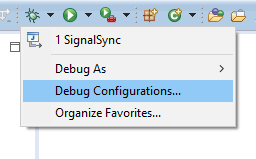
\includegraphics[width=0.3\textwidth]{debugconf.png}}
	\hfill
	\subfloat{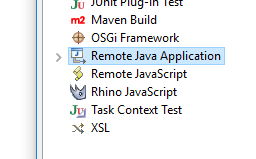
\includegraphics[width=0.3\textwidth]{debugremote.png}}
	\hfill
	\subfloat{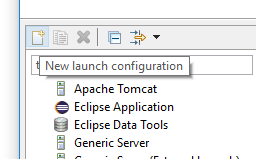
\includegraphics[width=0.3\textwidth]{debugnew.png}}
	\captionsetup{width=0.7\textwidth}
	\caption{Nieuwe debug configuration aanmaken in Eclipse}
	\label{debugconf}
\end{figure}

Ga hierna naar \textbf{Debug Configurations} in Eclipse. Selecteer \textbf{Remote Java Application} en klik vervolgens op het icoon van \textbf{new launch configuration}. Deze stappen worden verduidelijkt in figuur \ref{debugconf}.

\begin{figure}[!tbph]
	\captionsetup{width=0.7\textwidth}
	\caption{De debug configuratie in Eclipse}
	\begin{center}
		\advance\parskip0.3cm
		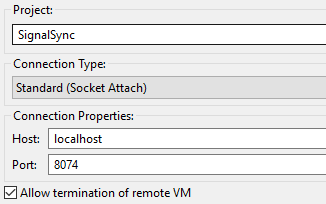
\includegraphics[width=0.5\textwidth]{debugsettings.png}
	\end{center}
	
	\label{debugsettings}
\end{figure}

Geef vervolgens de configuratie een naam en blader bij \textbf{Project} naar het te debuggen project (SignalSync). Kies bij \textbf{Connection Type} voor \textbf{Standard (Socket Attach)}. Bij \textbf{Connection Properties} moet de poort worden opgegeven die in het Max/MSP configuratiebestand gespecificeerd is (standaard 8074). Aangezien de applicatie lokaal draait moet bij \textbf{Host} \texttt{localhost} of \texttt{127.0.0.1} worden opgegeven. Met \textbf{Allow termination of remote VM} kan worden ingesteld of de Max/MSP VM vanuit Eclipse mag worden afgesloten. Figuur \ref{debugsettings} toont een screenshot van de instellingen.

Het debuggen wordt gestart door eerst de Max/MSP patch te openen en vervolgens het debuggen in Eclipse te starten met de zojuist aangemaakt debug configuratie. Bij het starten van de patch is het nu mogelijk om via breakpoints door de code navigeren.

\subsection*{Genereren van testdata}

De bestanden die vereist zijn voor het uitvoeren van de testen bevinden zich niet in het GitHub repository maar moeten nog gegenereerd worden. 

De eerste stap voor het genereren van de bestanden is het uitvoeren van het Perl script \texttt{TestSetGenerator.pl}. Dit script kan gedownload worden van de map \textbf{Scripts} in het GitHub repository. Het script maakt van een groep mp3-bestanden verschillende varianten aan (zie \ref{latency-test} en \ref{sine-test}). In het script moet de bron- en doelmap worden opgegeven.

Met behulp van de Java applicatie \texttt{SlicerApp} uit de package \texttt{be.signalsync.app} kunnen de gegenereerde bestanden worden omgezet in slices. Deze slices dienen als input voor enkele testen.


